\subsubsection{TENT} \label{sssec:tent}

\textcolor{red}{The equation that represents the implementation for $u=2$ is:} 
%
\begin{equation}\label{eq:tent2B2}
x_{n+1} = 
\begin{cases}
2~x_n &, \textrm{if } 0\leq x_n\leq 0.5\\
\epsilon ~\text{floor} \{\frac{1}{\epsilon} 2~(1-x_n)\} &, \textrm{if } 0.5<x_n\leq 1 
\end{cases}	
\end{equation}
%
\textcolor{red}{Rounding is necessary only on the second multiplication} because it is equivalent to a shift-to-left.

When this map is implemented \textcolor{red}{with $u=2$} in any computer using any numerical representation system (even floating-point!) truncation errors rapidly increase and make the unstable fixed point in $x^*=0$ to become stable.
The sequences within the attractor domain of this fixed point will have a short transitory of length between $0$ and $B$ followed by an infinite number of $0$'s \cite{Jessa2002,Callegari}.
This issue is easily explained in \cite{Li2004}, the problem appears because all iterations have a left-shift operation that carries the $0$'s from the right side of the number to the most significant positions.
\textcolor{red}{As expected, the quantifiers} $H_{hist}$, $H_{BP}$ and $C_{BP}$ are equal to zero for all precisions.
In the case of $H_{BPW}$ and $C_{BPW}$ quantifiers are different to zero because BPW procedure discards the elements once the fixed point is reached.
$H_{BPW}$, $C_{BPW}$ and MP present high dispersions related to the short length of serie's transient.
These transients have a maximum length of $B$ elements (iterations) for fixed-point arithmetic and $53$ for floating-point (IEEE754 double precision).

Figures \ref{fig:Hval_Tent} to \ref{fig:MP_Tent} show the quantifiers for floating- and fixed-point numerical representations \textcolor{red}{for $u=1.96$.}
\textcolor{red}{The results are similar to those of the LOG map, in that the averaged value of the quantifiers tends not monotonously to the floating point value and stabilizes from a certain value of $B$.
However, more bits of precision were necessary to achieve this, on the other hand it can be seen that the value of $H_ {hist}$ improves and that of $H_ {BP}$ remains similar to those of the LOG map.
Using $H_ {BPW}$ and $C_ {BPW}$ we detect that below the $13$ precision bits some initial conditions converge to fixed points or diverge, so it is not possible to use this map with $B <13$.}
%
\begin{figure}[H]
	\centering
	\begin{subfigure}[b]{0.49\textwidth}
		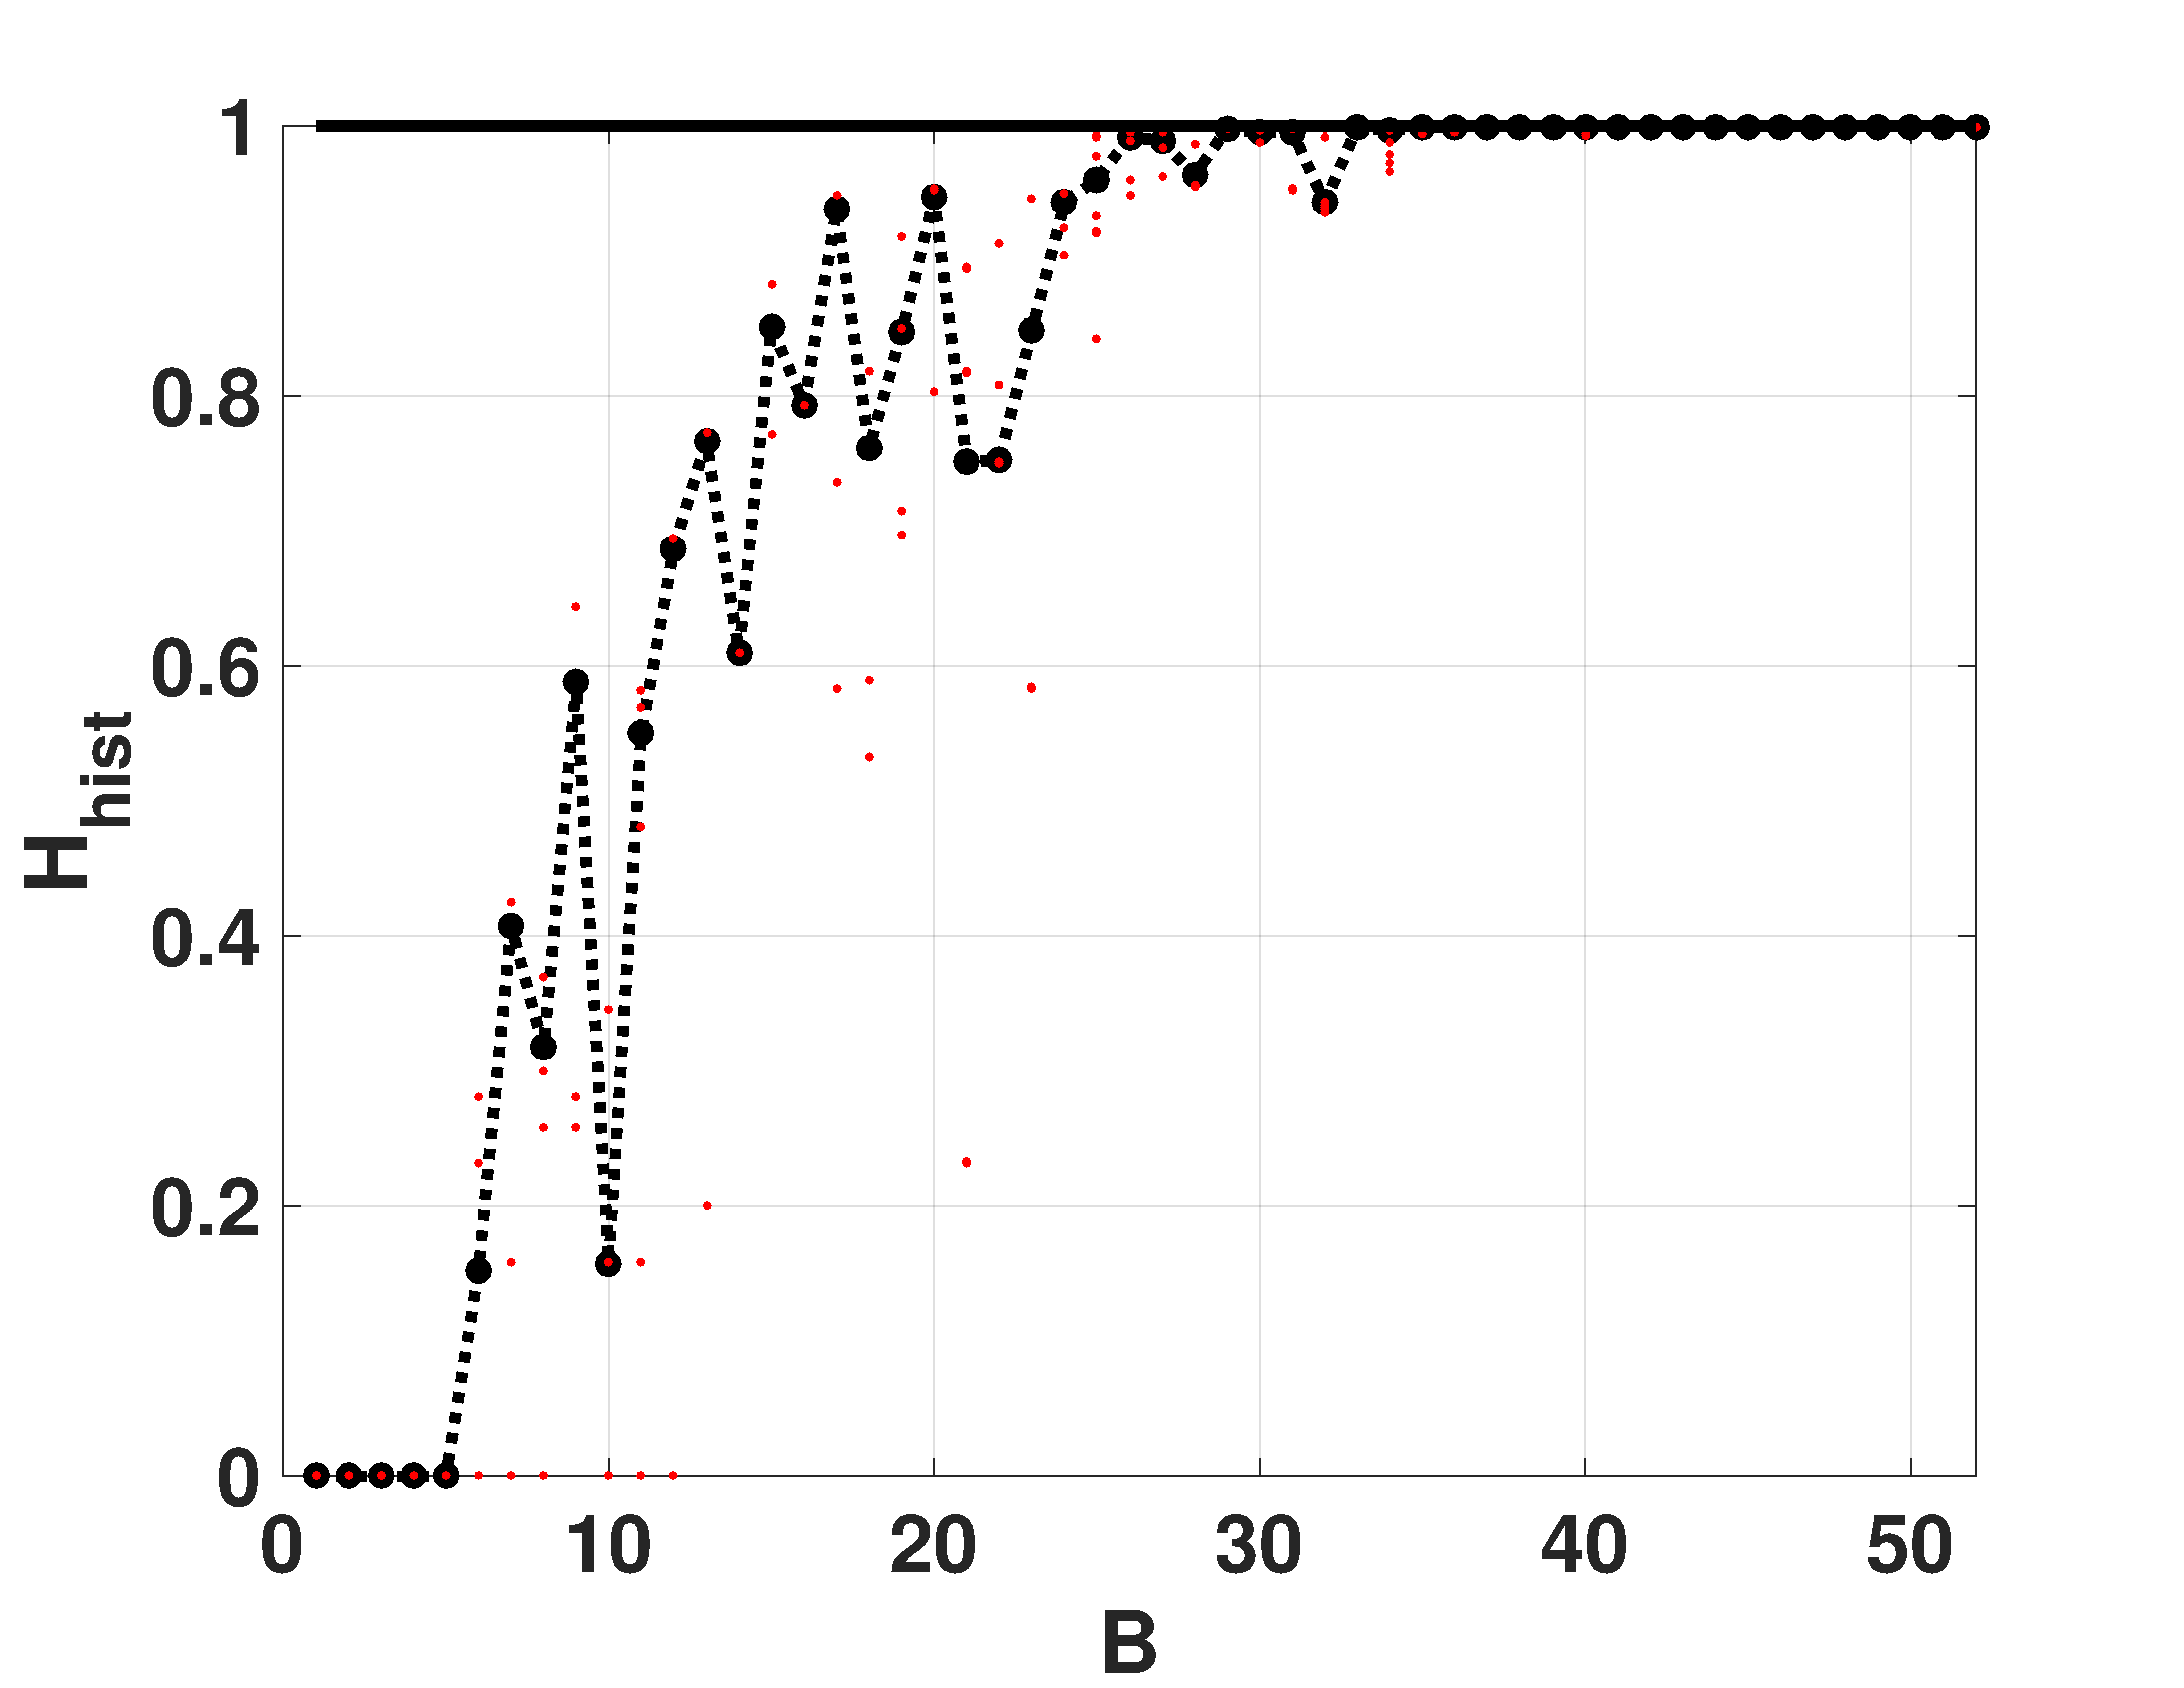
\includegraphics[width=\textwidth]{Hval_Tent1p96}
		\caption{$H_{hist}$ vs. $B$}
		\label{fig:Hval_Tent}
	\end{subfigure}
	\begin{subfigure}[b]{0.49\textwidth}
		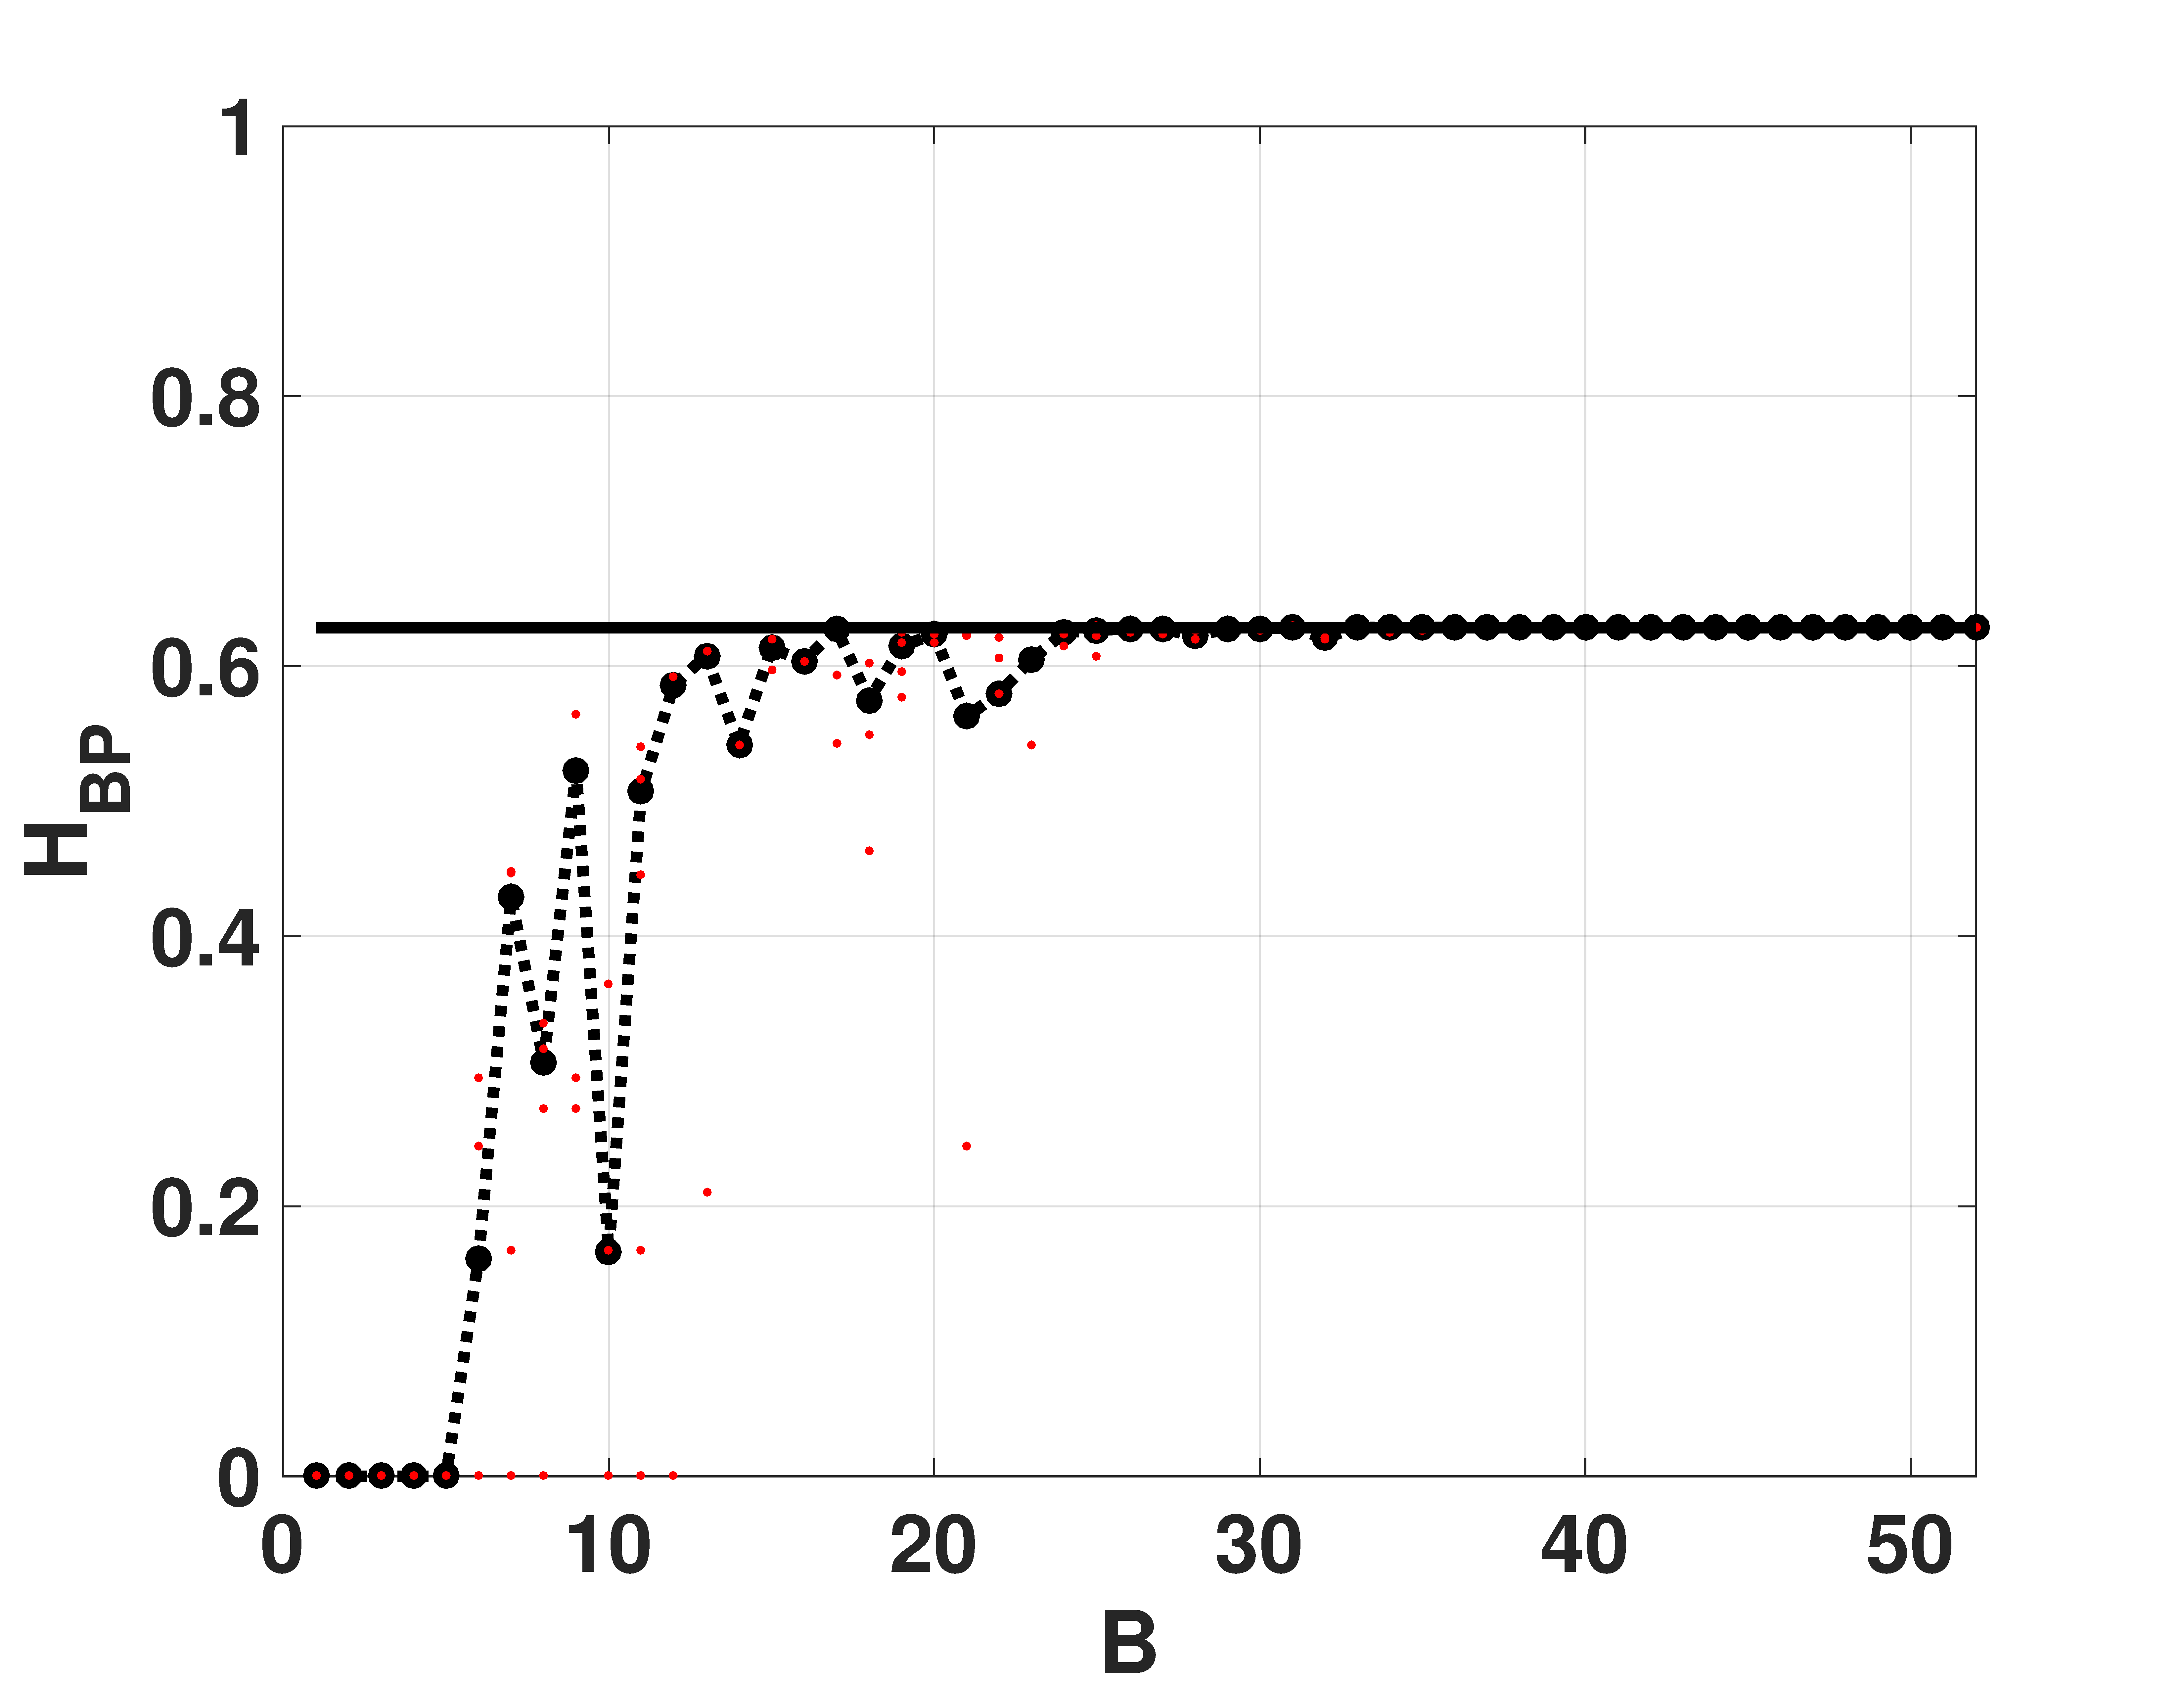
\includegraphics[width=\textwidth]{Hbp_Tent1p96}
		\caption{$H_{BP}$ vs. $B$}
		\label{fig:Hbp_Tent}
	\end{subfigure}
	\begin{subfigure}[b]{0.49\textwidth}
		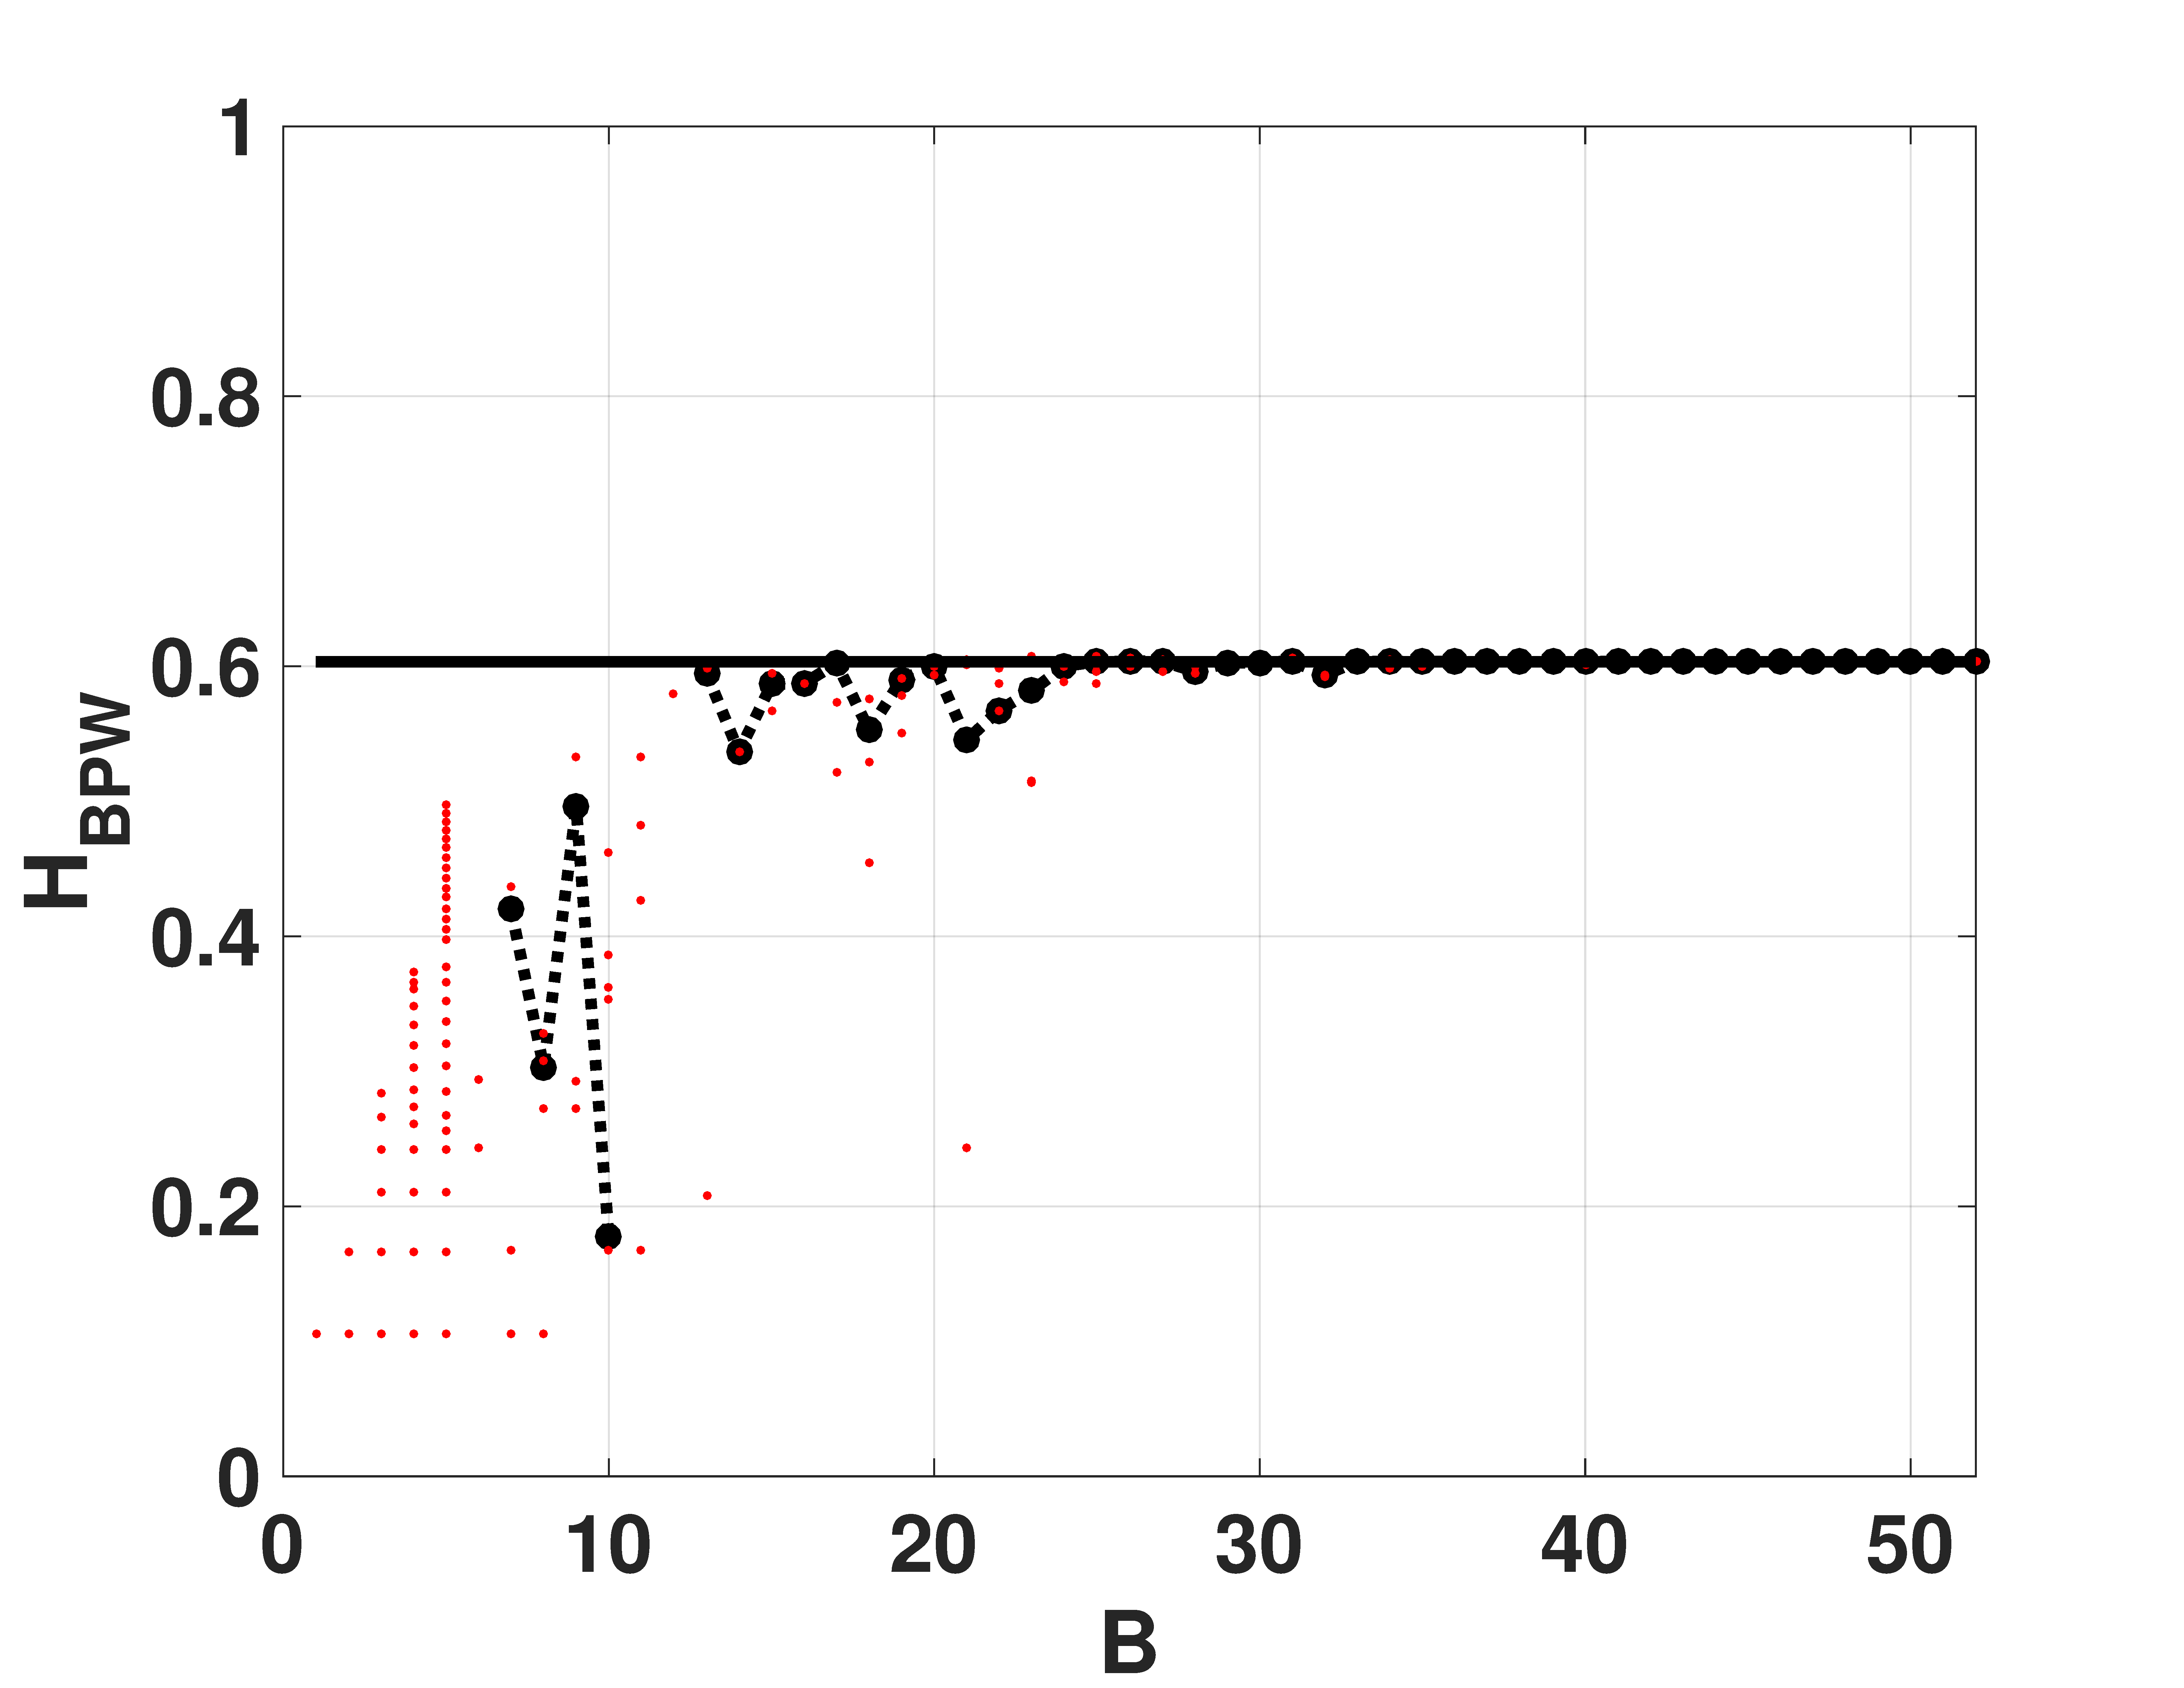
\includegraphics[width=\textwidth]{Hbpw_Tent1p96}
		\caption{$H_{BPW}$ vs. $B$}
		\label{fig:Hbpw_Tent}
	\end{subfigure}
	\begin{subfigure}[b]{0.49\textwidth}
		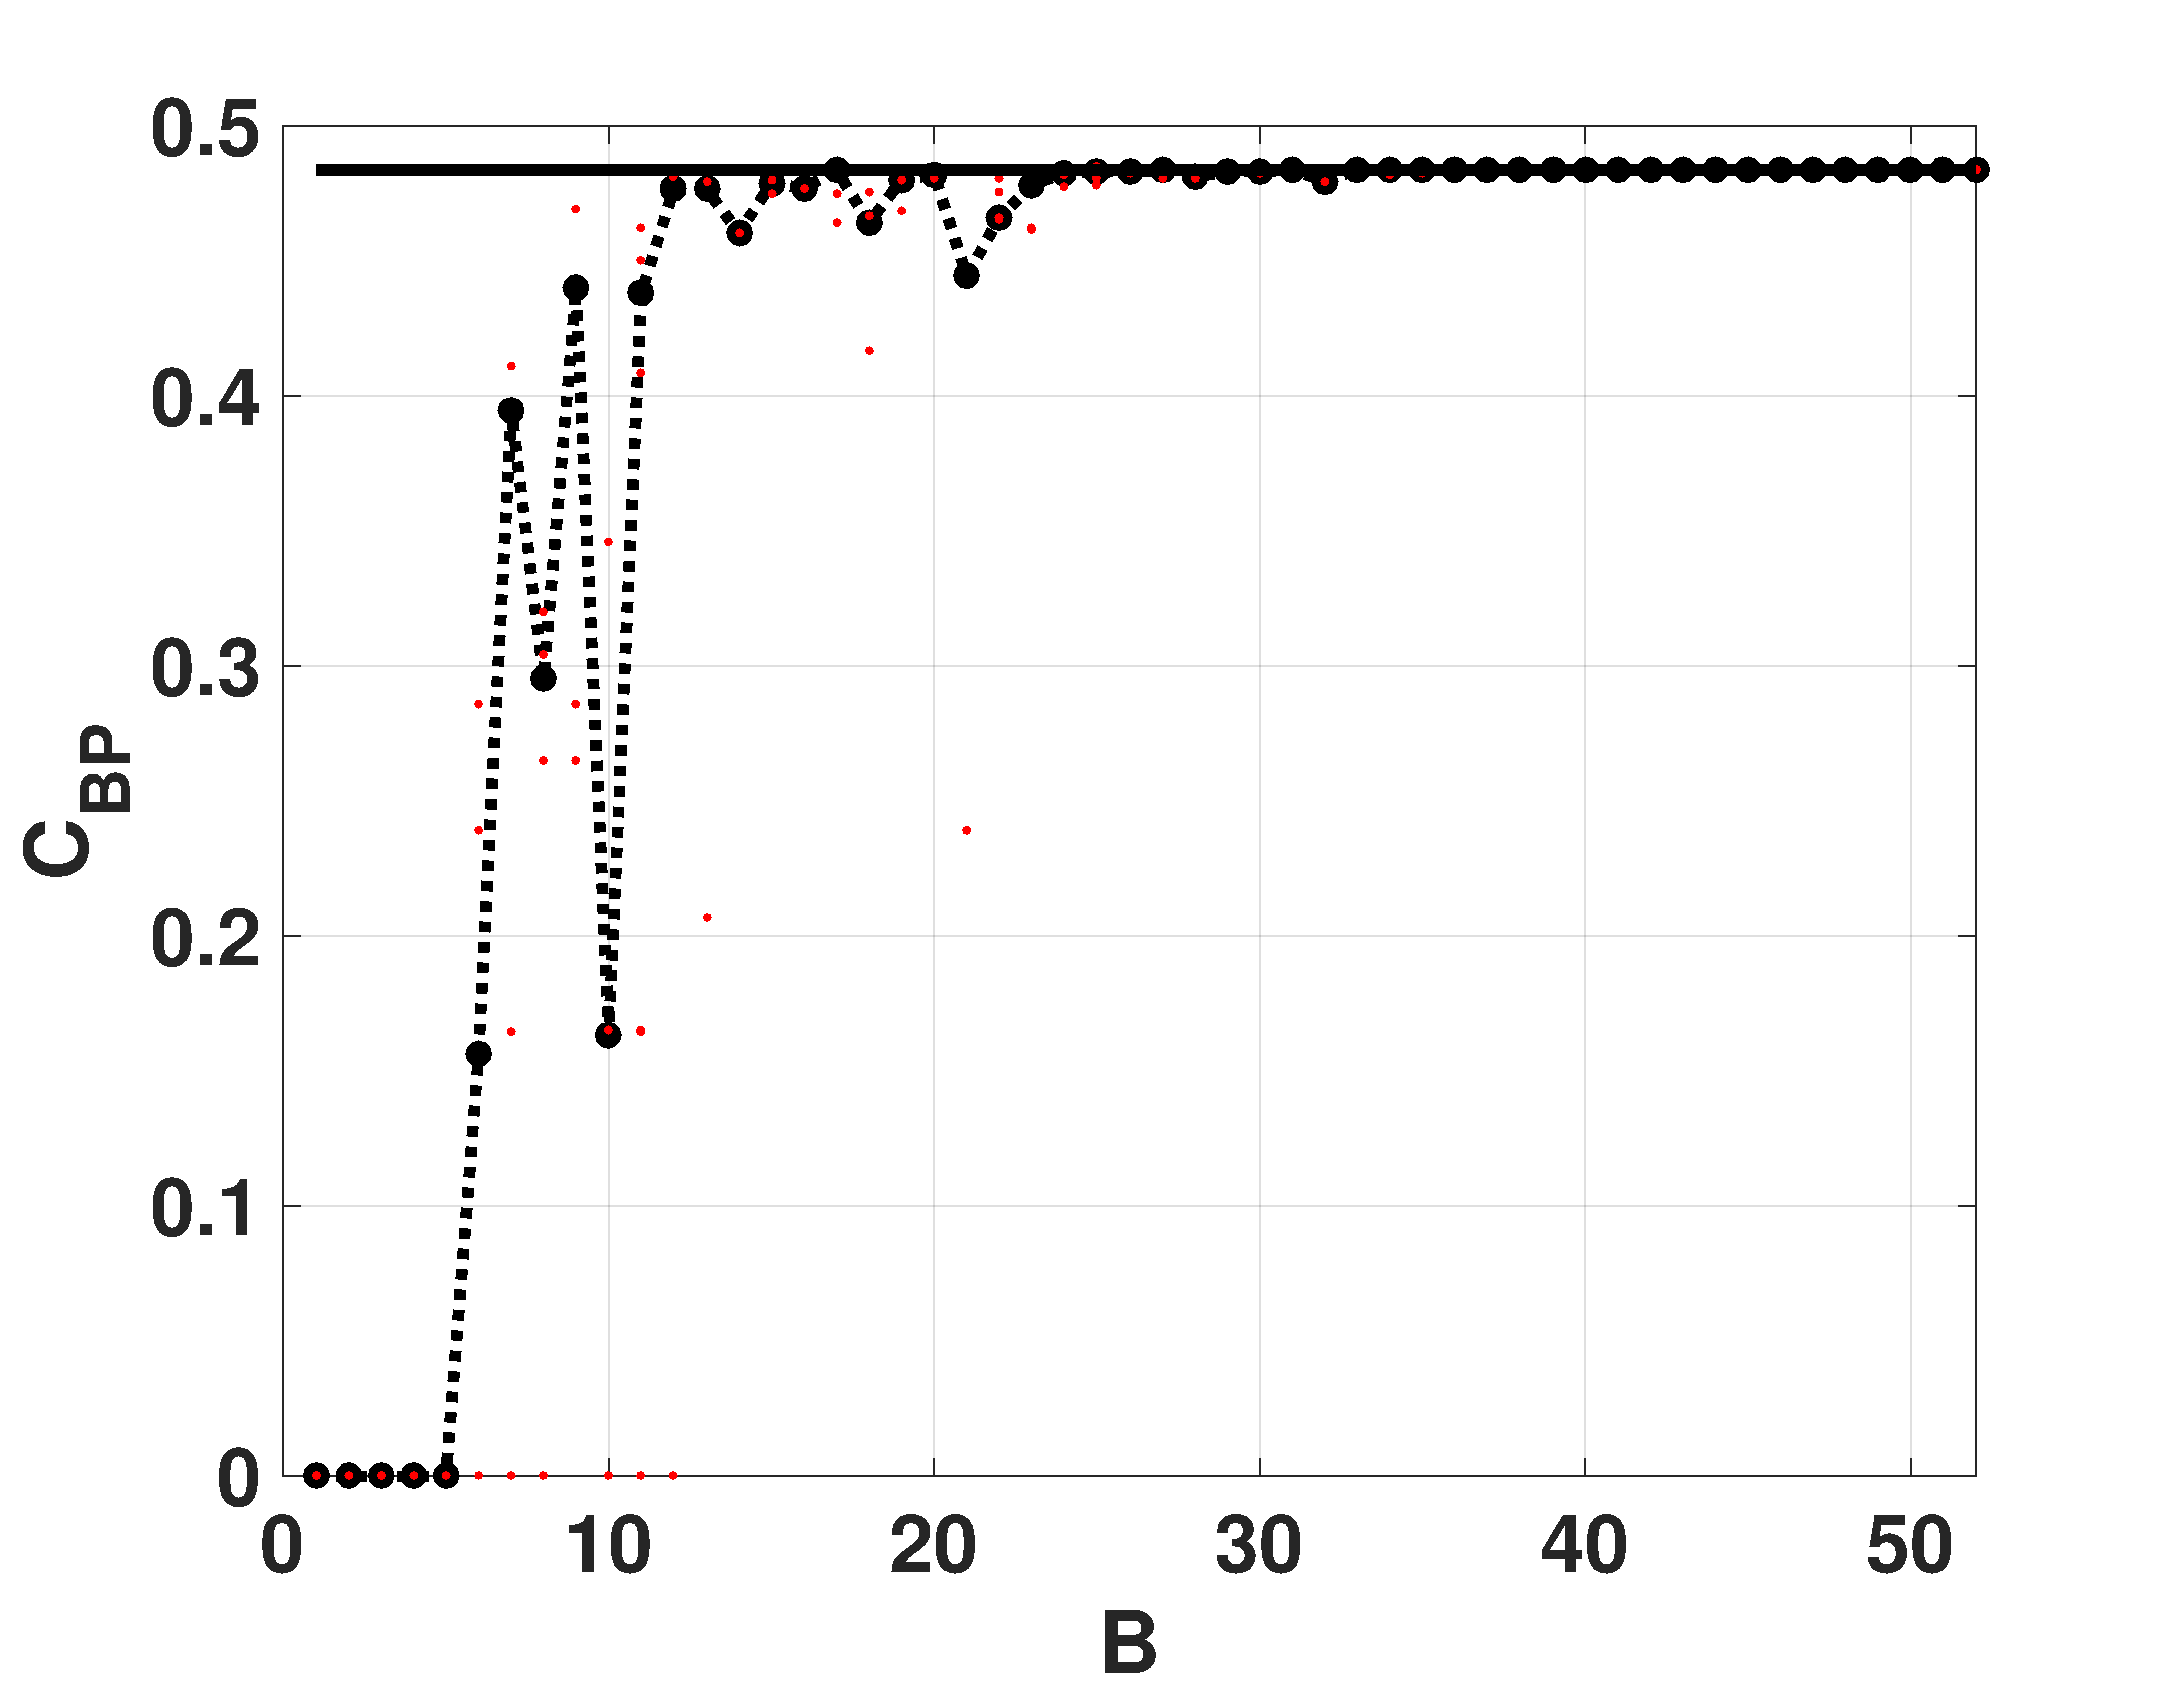
\includegraphics[width=\textwidth]{Cbp_Tent1p96}
		\caption{$C_{BP}$ vs. $B$}
		\label{fig:Cbp_Tent}
	\end{subfigure}
	\begin{subfigure}[b]{0.49\textwidth}
		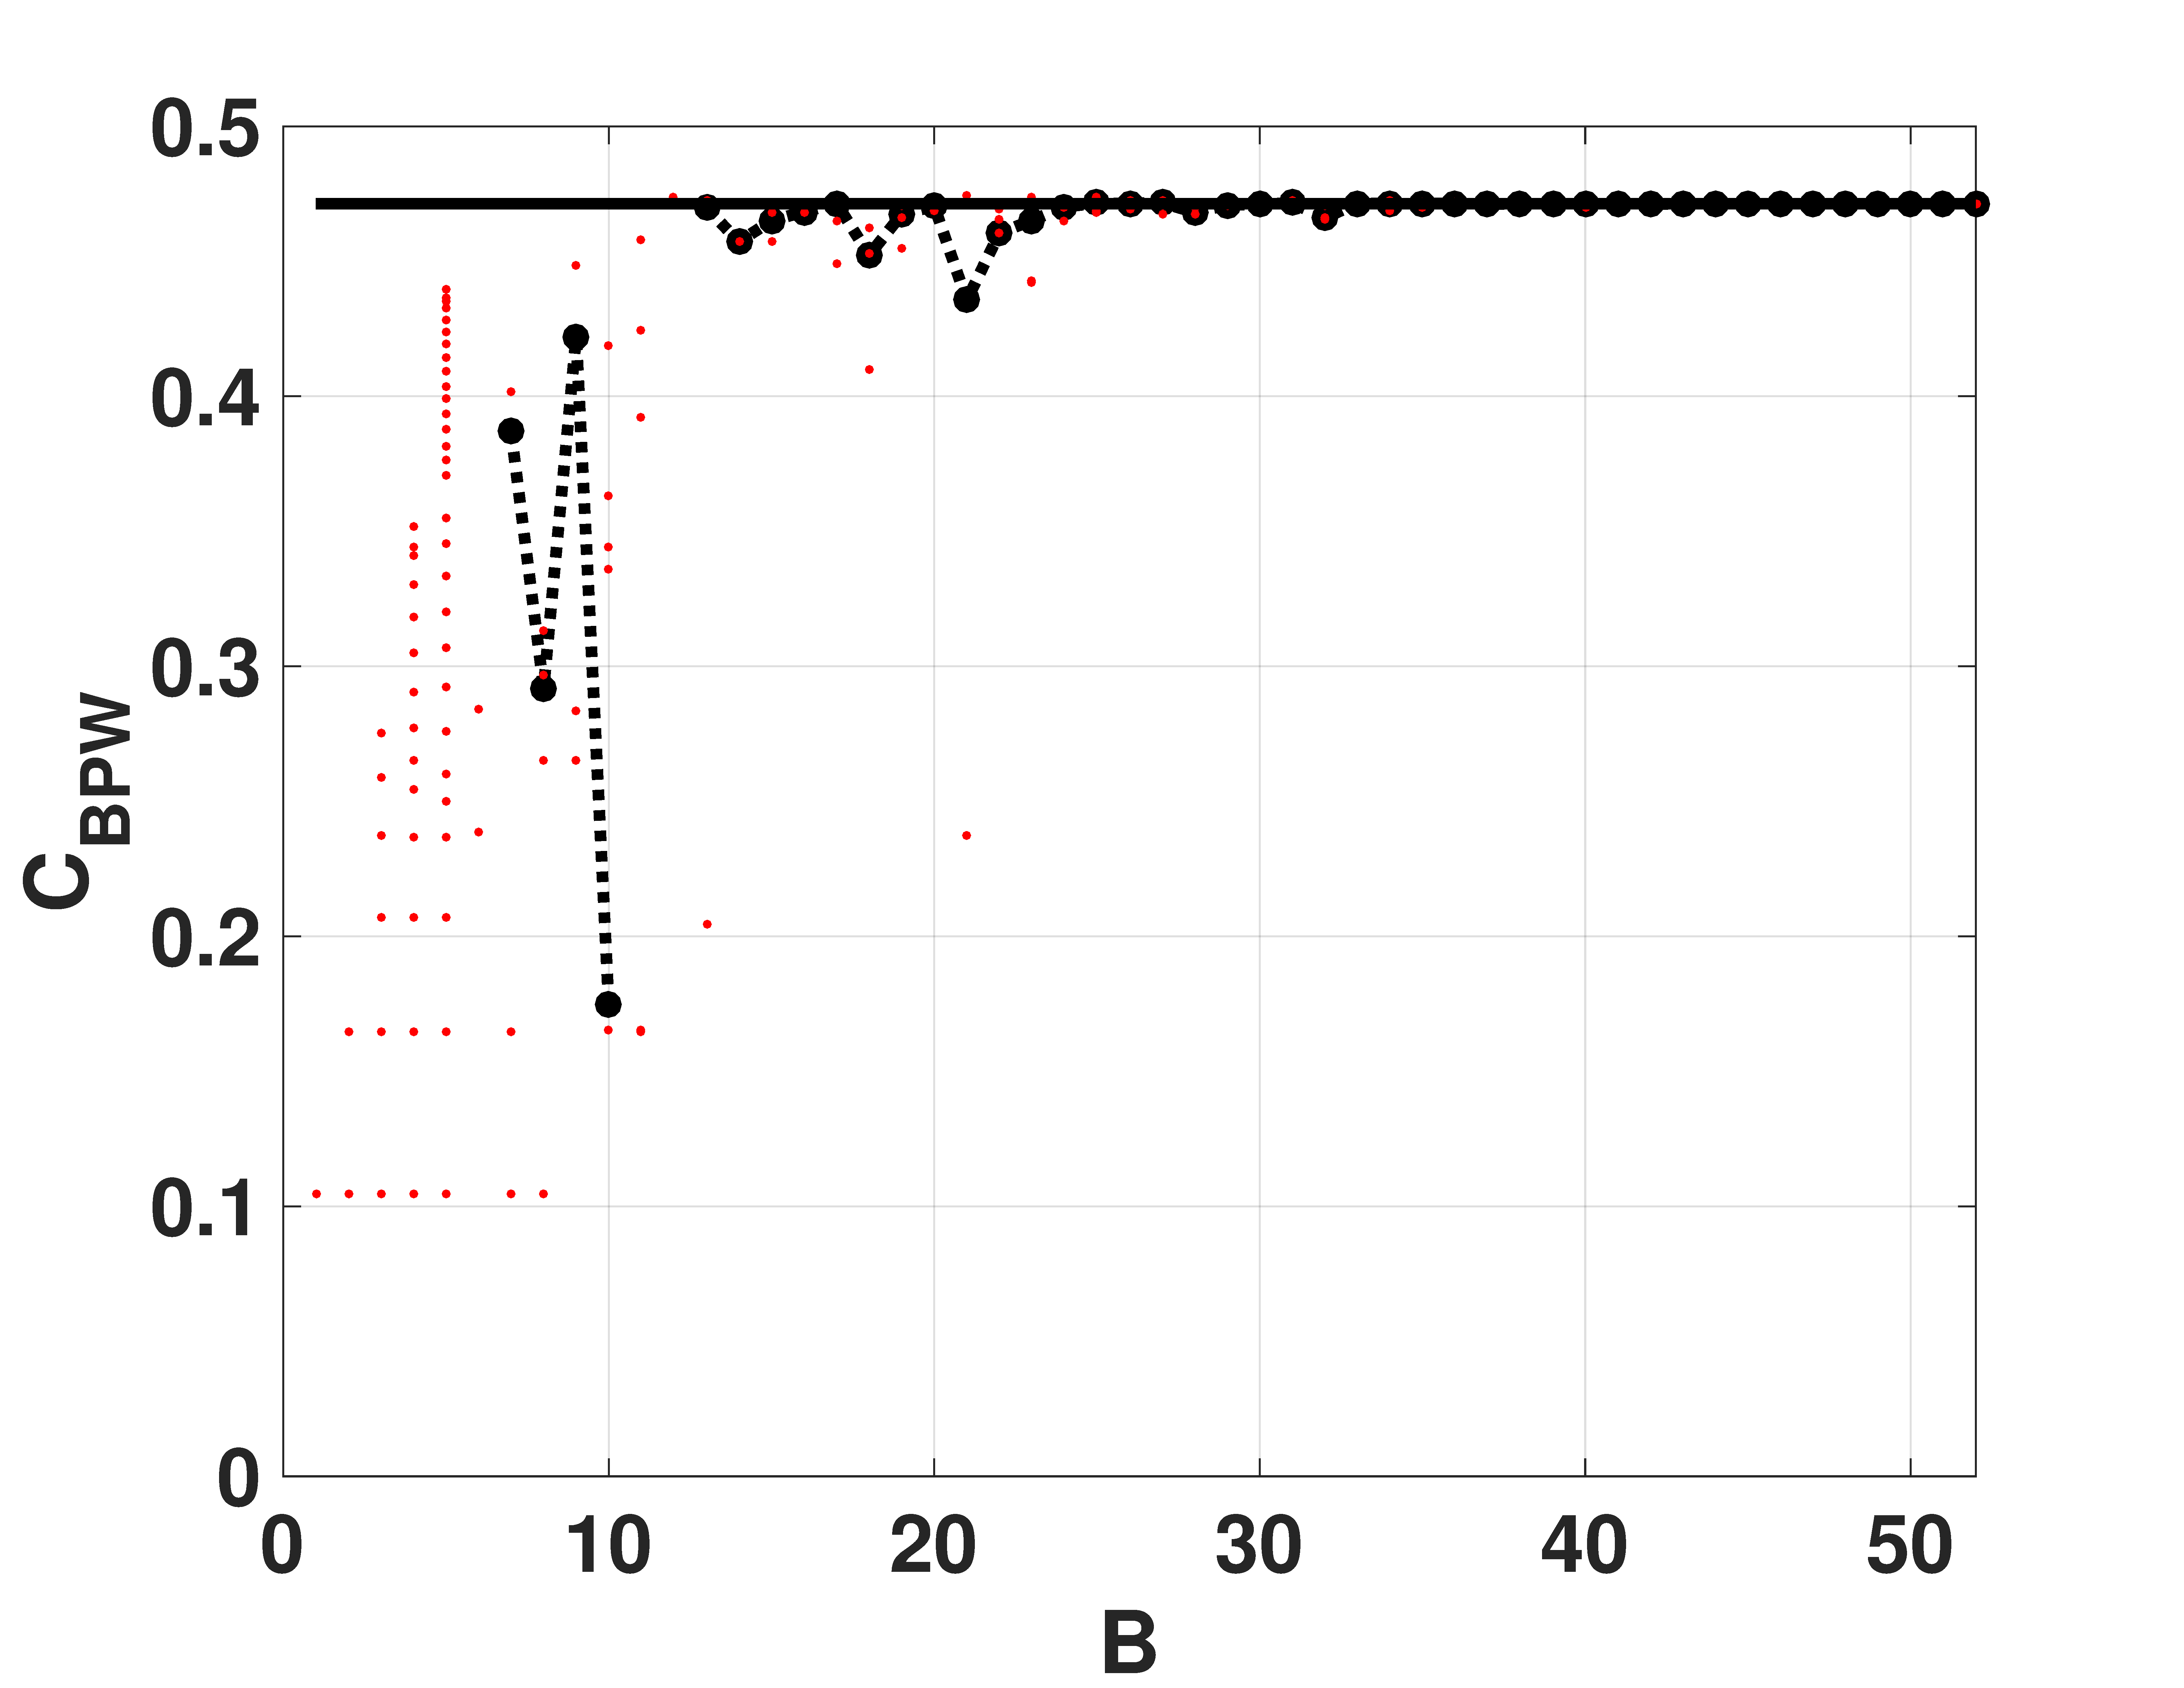
\includegraphics[width=\textwidth]{Cbpw_Tent1p96}
		\caption{$C_{BPW}$ vs. $B$}
		\label{fig:Cbpw_Tent}
	\end{subfigure}
	\begin{subfigure}[b]{0.49\textwidth}
		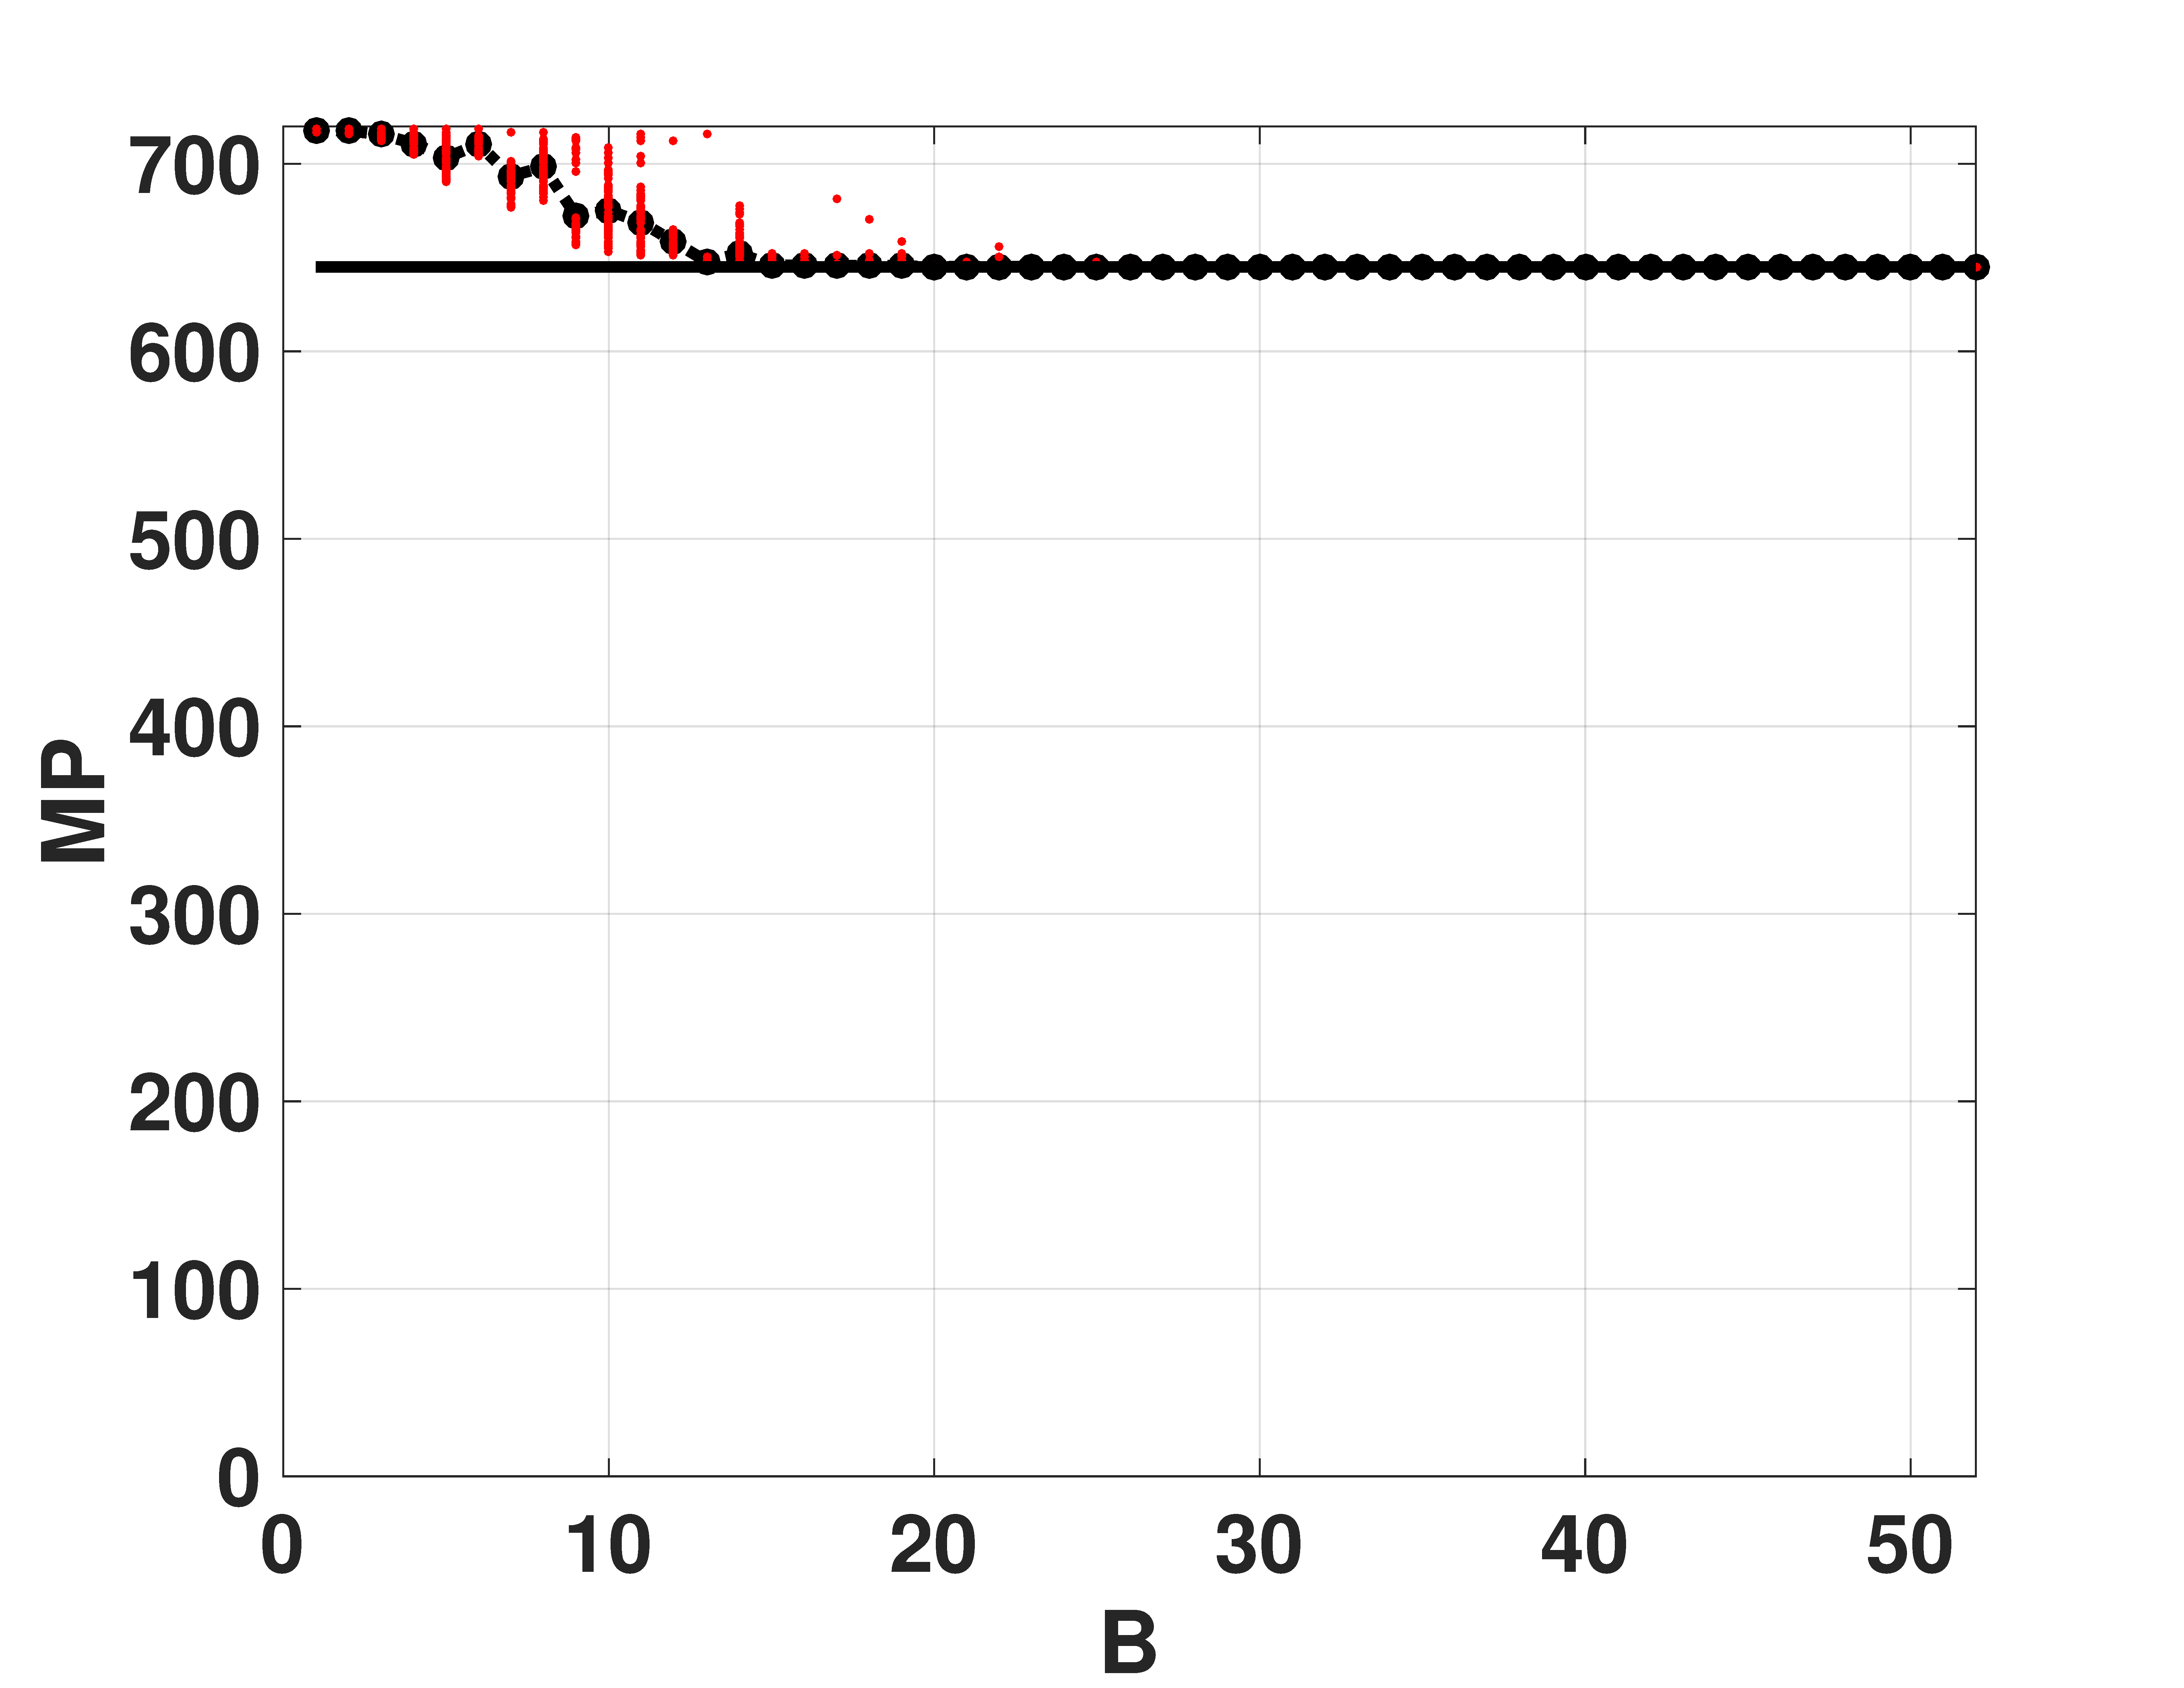
\includegraphics[width=\textwidth]{MP_Tent1p96}
		\caption{MP vs. $B$}
		\label{fig:MP_Tent}
	\end{subfigure}
	\caption{Statistical properties of TENT map \textcolor{red}{with paramater $u=1.96$}.}
	\label{fig:TENT_QuantiB}
\end{figure}

\textcolor{red}{The positions on the double entropy (Fig. \ref{fig:TENT1p96_HH}) and entropy complexity (Fig. \ref{fig:TENT1p96_HbpCbp}) planes are marginally better than those on the LOG map and are characteristic of a pseudo-chaotic system.}
%
\begin{figure}[H]
	\centering
	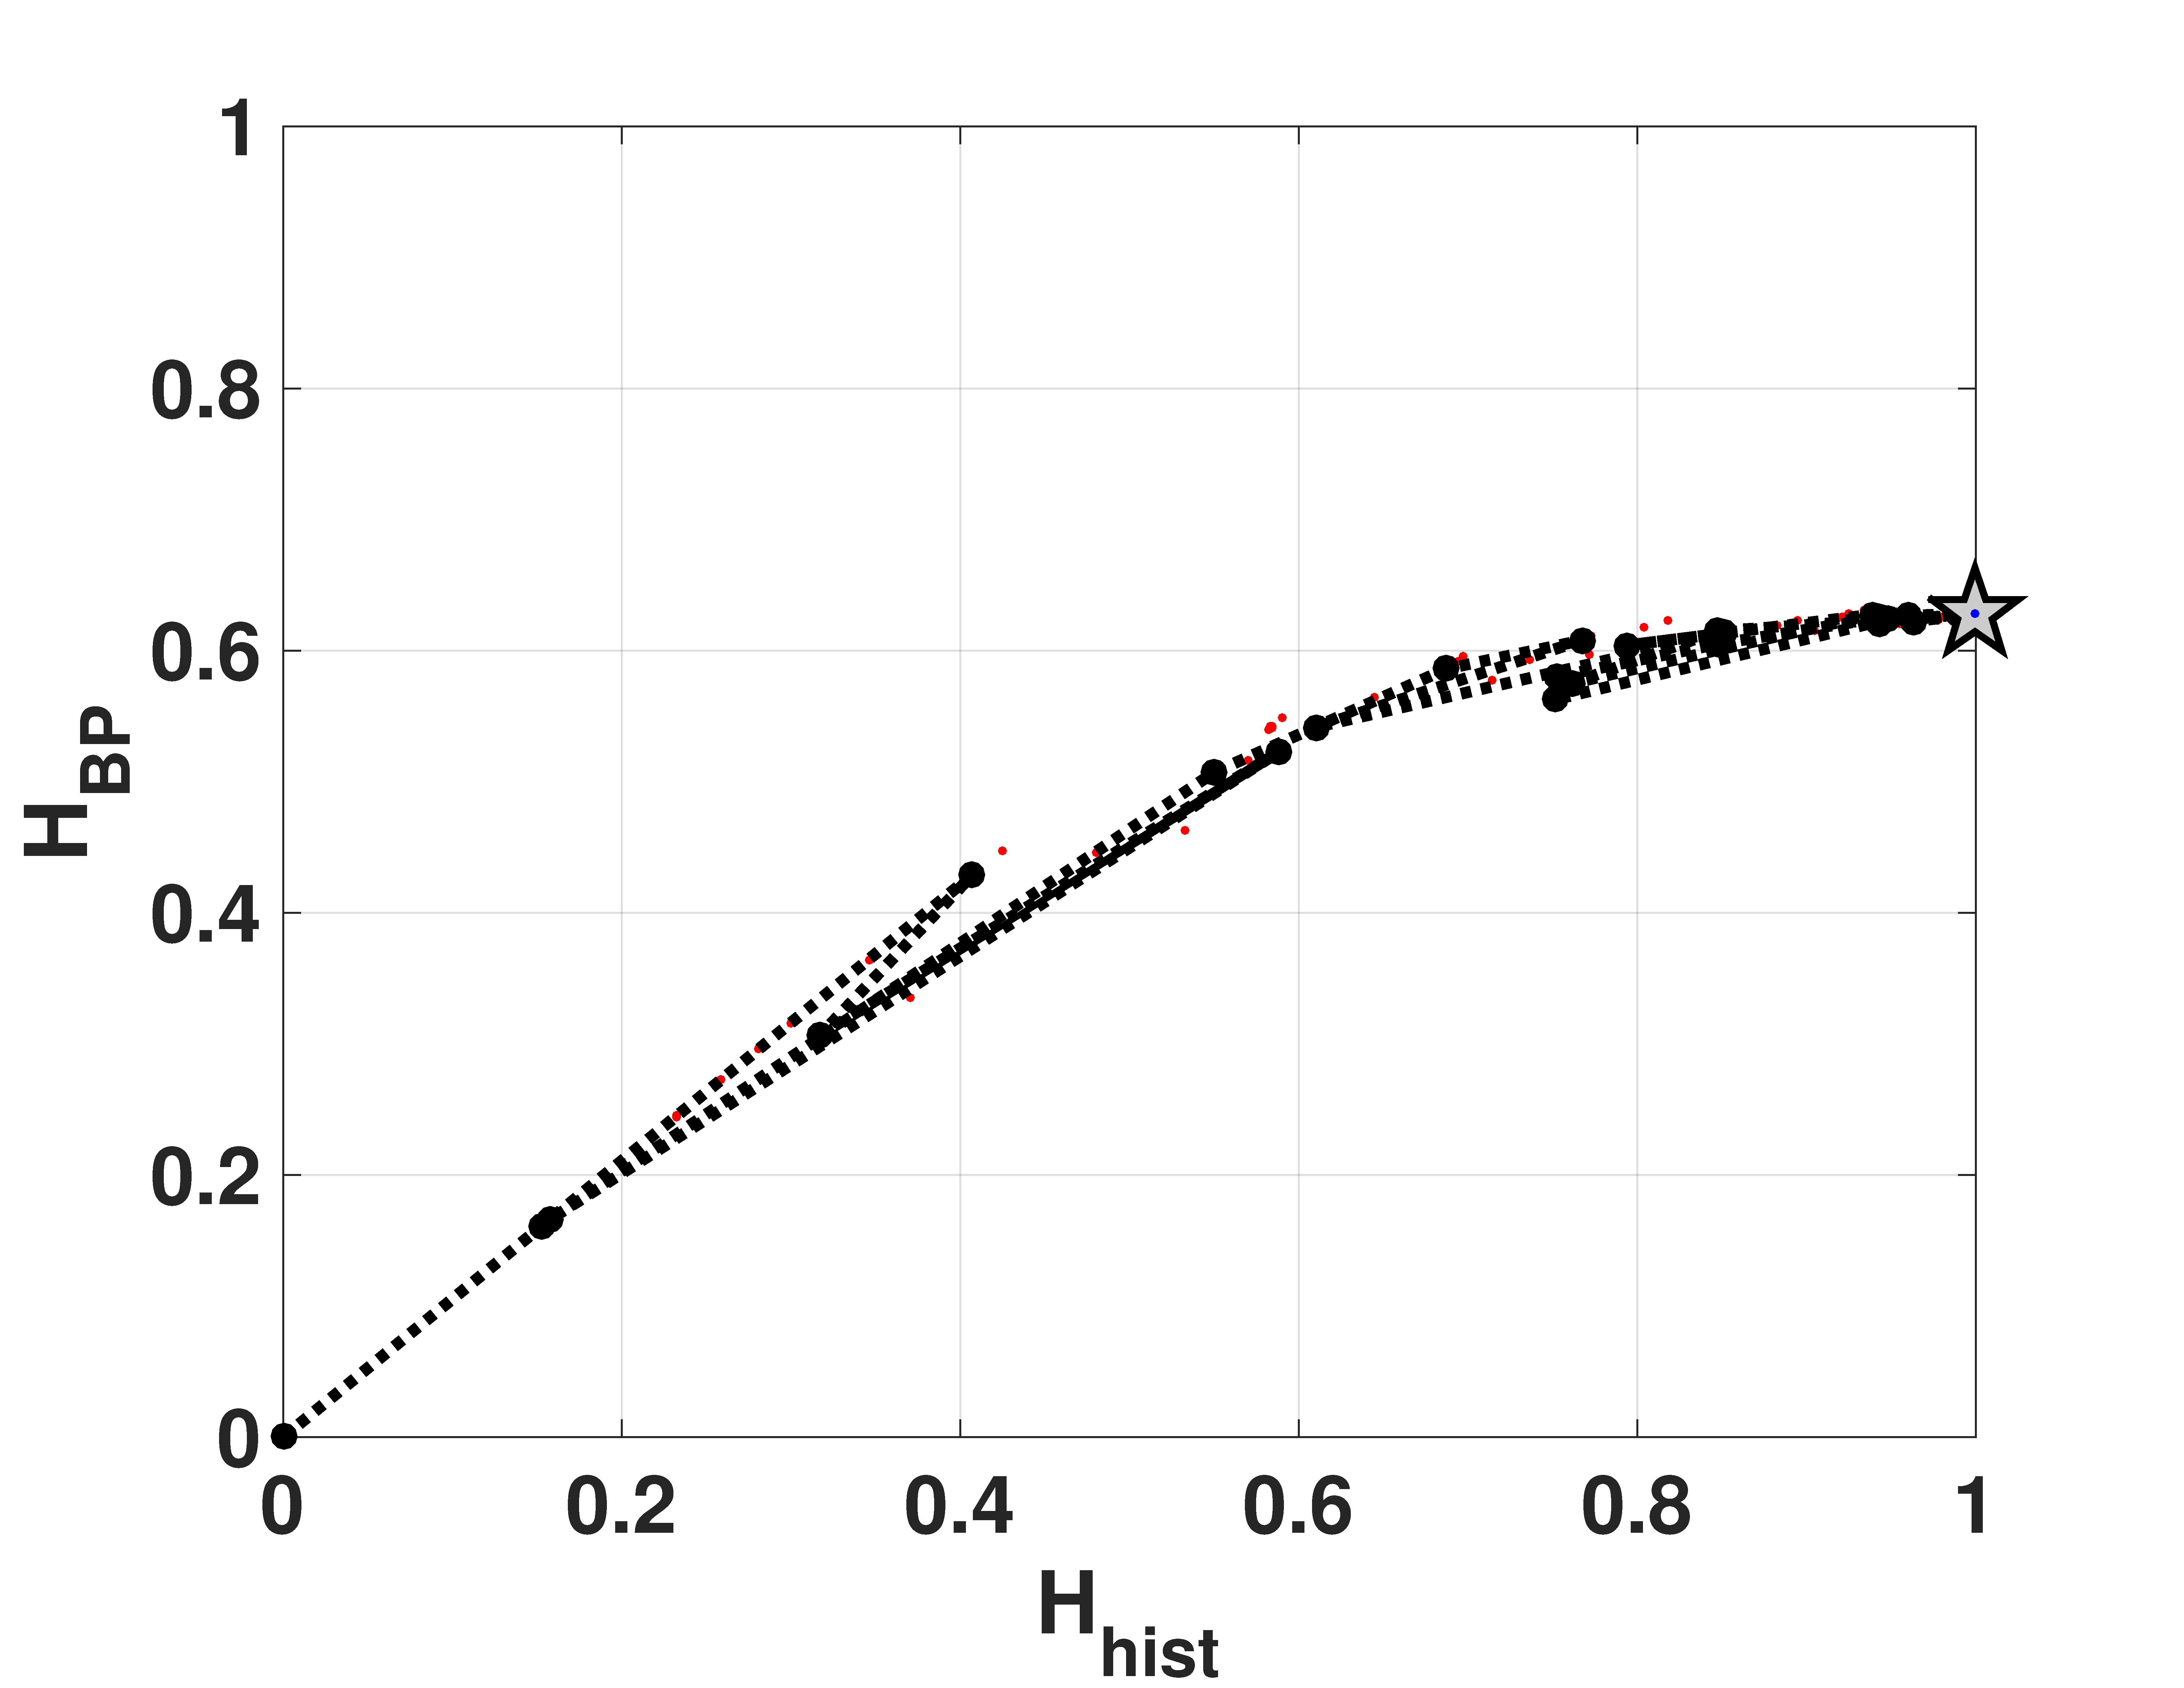
\includegraphics[width=.49\textwidth]{HbpHval_Tent1p96}
	\caption{Evolution of statistical properties in double entropy plane for TENT map with $u=1.96$.}
	\label{fig:TENT1p96_HH}
\end{figure}
%
\begin{figure}[H]
	\centering
	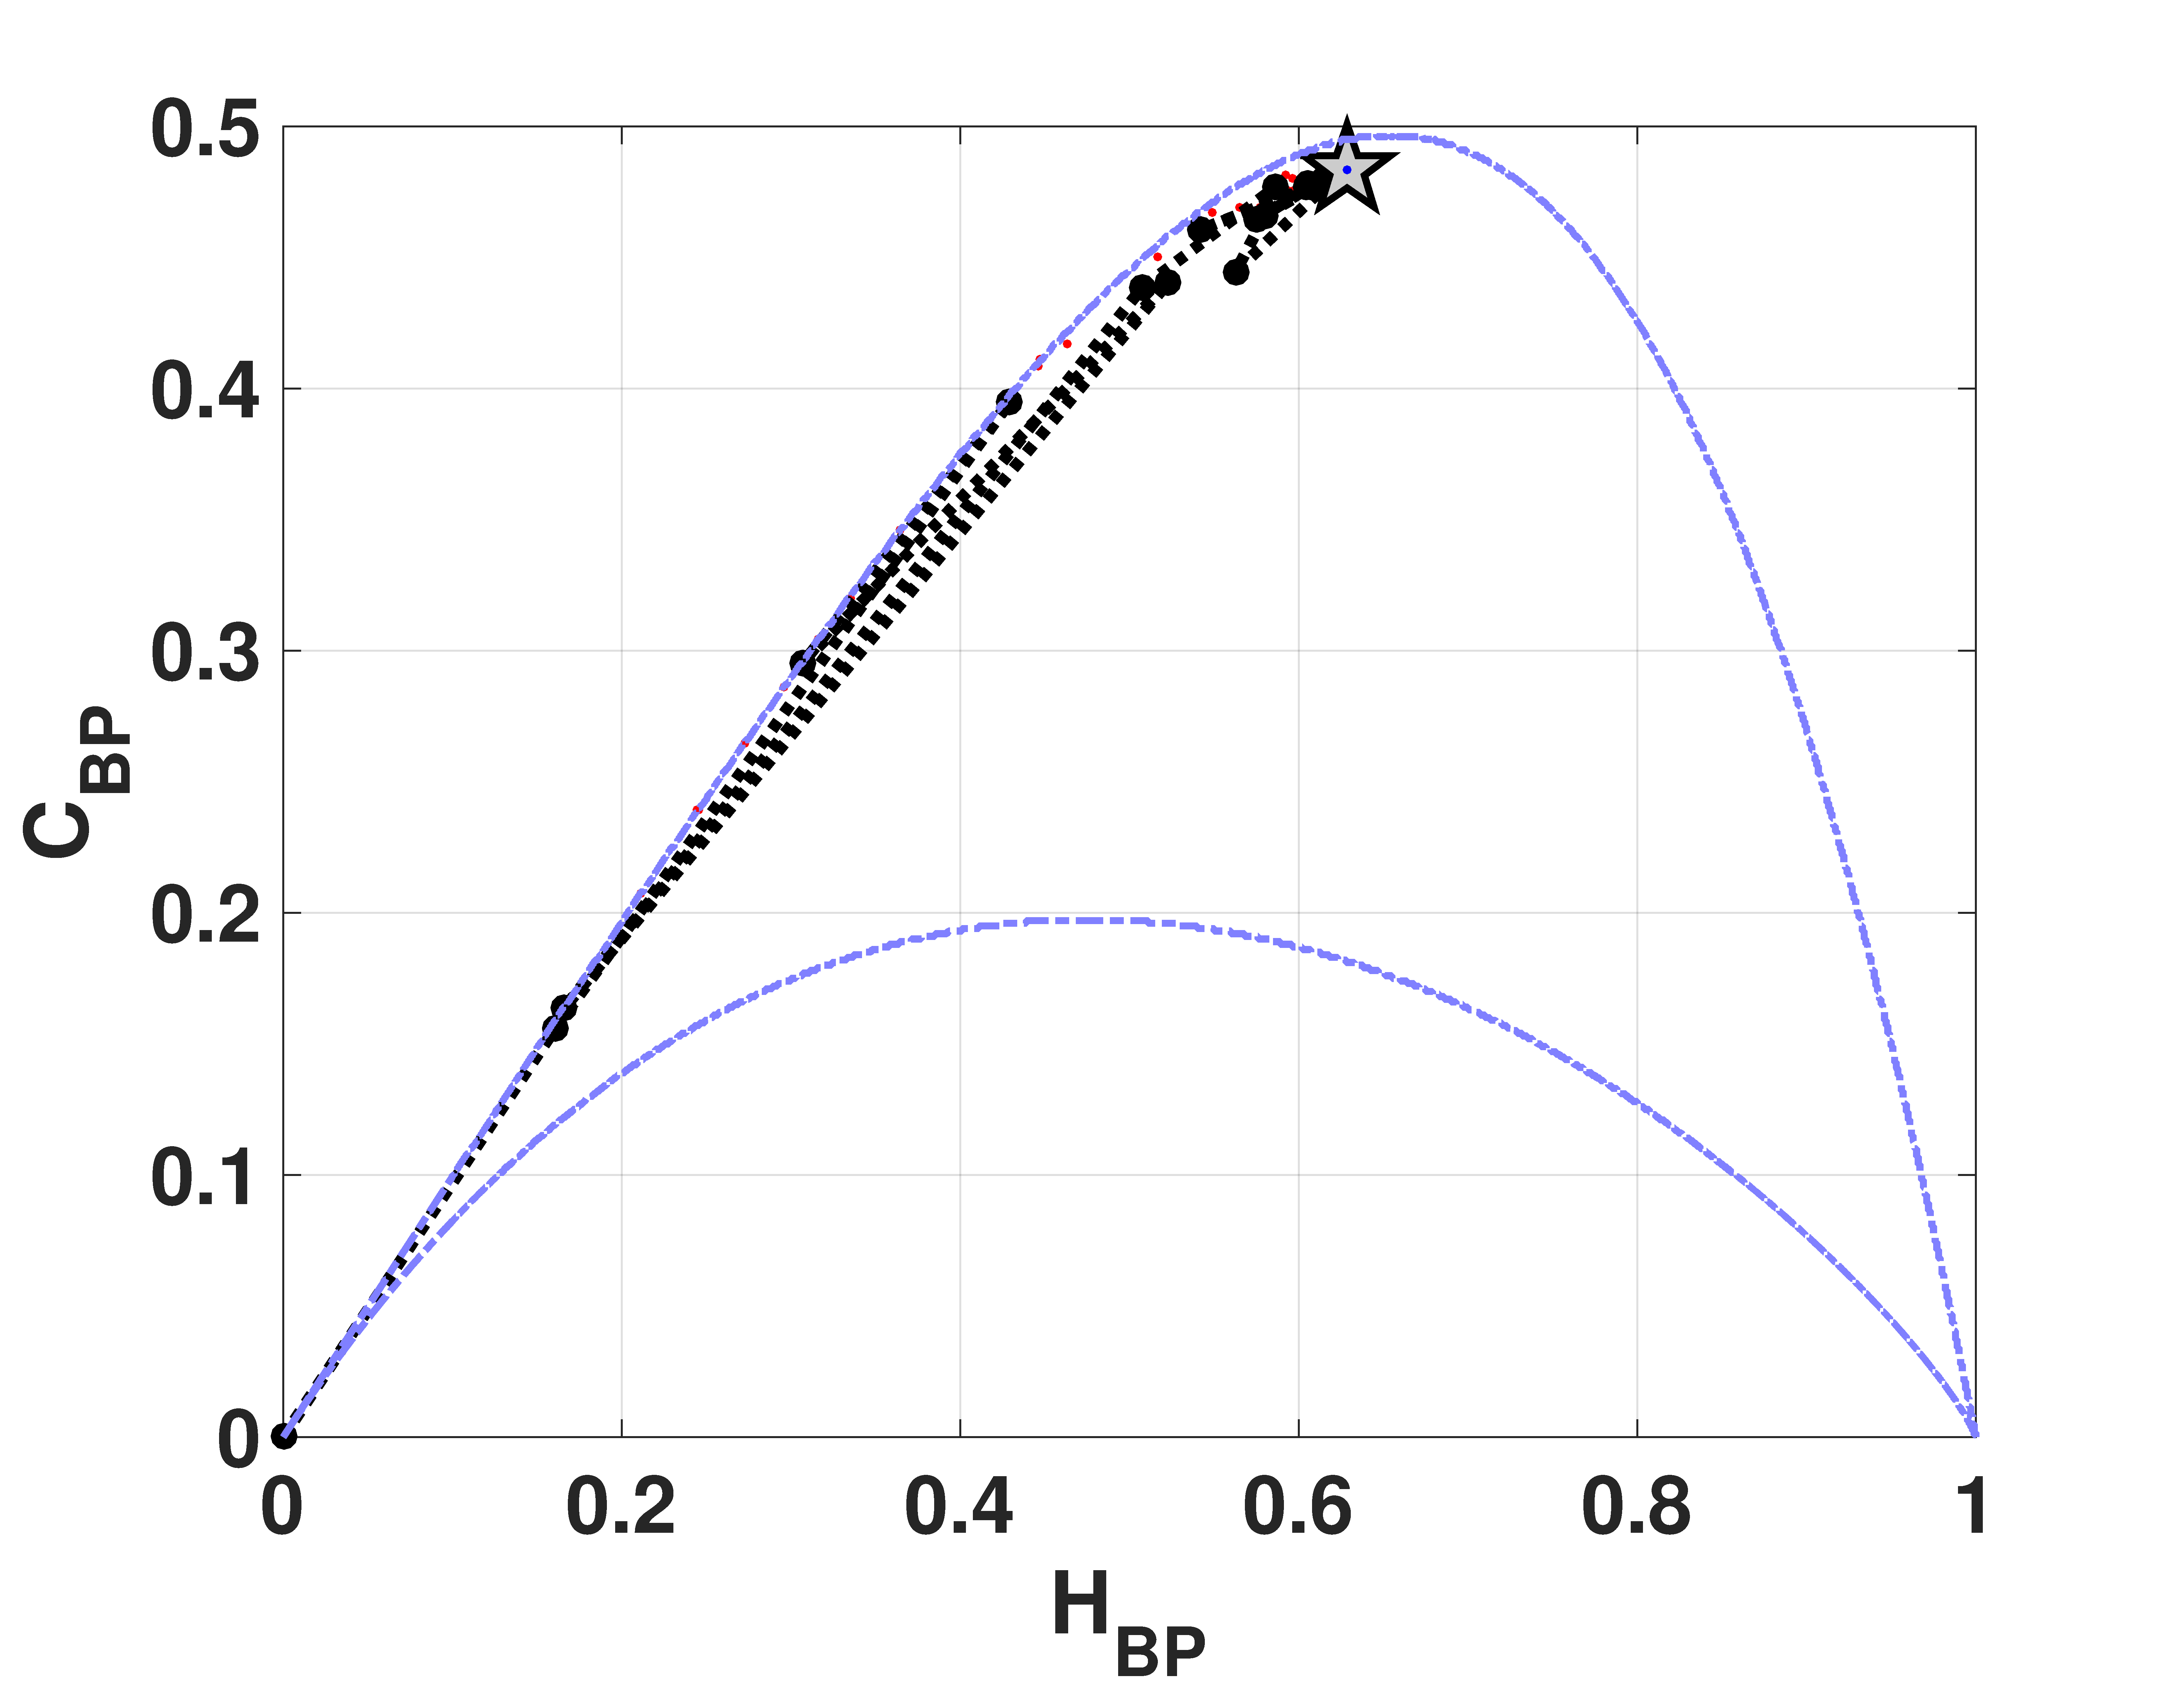
\includegraphics[width=.49\textwidth]{CbpHbp_Tent1p96}
	\caption{$H_{BP} \times C_{BP}$}
	\caption{Evolution of statistical properties in causal entropy-complexity plane for TENT map with $u=1.96$.}
	\label{fig:TENT1p96_HbpCbp}
\end{figure}